\thispagestyle{empty}

\begin{center} 

\large \textbf{R}épublique \textbf{A}lgérienne \textbf{D}émocratique et \textbf{P}opulaire\\
\textbf{M}inistère de\textbf{ l}’Enseignement \textbf{S}upérieur et de la\textbf{ R}echerche \textbf{S}cientifique\\
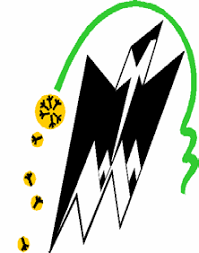
\includegraphics[width=0.1\textwidth]{pdg/ummto.png}\\
\textbf{U}NIVERSITÉ \textbf{M}OULOUD \textbf{M}AMMERI DE \textbf{T}IZI-OUZOU\\
\textbf{ FACULTE DE GENIE ÉLECTRIQUE ET DE L’INFORMATIQUE}\\\vfill


\end{center}


\begin{center}
    \huge Module:Architechture Logiciel\normalsize\\
 
    \rule{0.90\textwidth}{2pt}\\
    \LARGE \textbf
    {Présentation de la technologie \textbf{CORBA}}\\
    \normalsize
    \rule{0.90\textwidth}{2pt}\\
    \large INGÉNIERIE DES SYSTÈMES D'INFORMATION \\
    \vfill
    \begin{flushright}
     \large \textbf {Pr: M.KERBICHE} \\
    \end{flushright}
  \vfill
\begin{flushleft}   
 \large\emph{\textbf{NOM ET PRENOM:}}
 \begin{itemize}[label=$\bullet$]
      \item AIT-IKENE Nadjib
      \item BOUCHERK Salim
      \item BOUSSAKOU Noureddine
      \item KACETE Djouher
      \item HADJ NACEUR Rayane
      \item TIGHREMT Zineb
 \end{itemize}
\end{flushleft}
\vfill

\begin{flushright}
\large Année Universitaire: 2022/2023\\
\end{flushright}
   
\end{center}
    
%\end{document}